\subsection{UC9 - Verifica dello stato di \glossario{Check-in}/Check-out}
\begin{itemize}
	\item \textbf{Identificativo}: UC9
	\item \textbf{Nome}: Verifica dello stato di \glossario{Check-in}/Check-out
	\item\textbf{Descrizione Grafica}: 
	
	\begin{figure}[h]
		\centering
		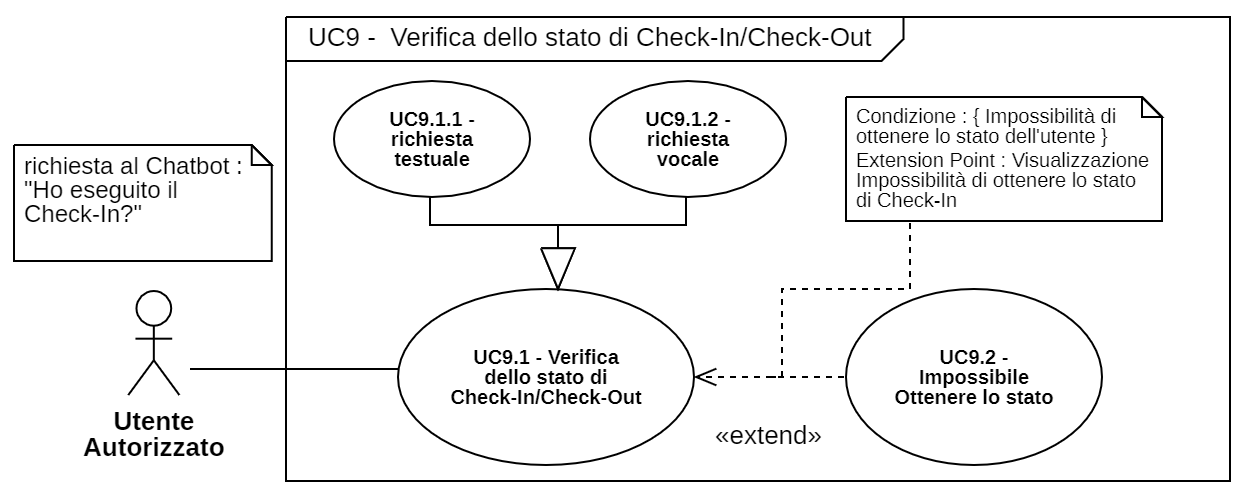
\includegraphics[scale=0.60]{images/UC9.png} 
		\caption{Descrizione grafica caso d'uso UC9}
	 \end{figure}

	\item \textbf{Attori}
	\begin{itemize} 
		\item \textit{Primari}: Utente autorizzato
		\item \textit{Secondari}: Non presenti
	\end{itemize}
	\item \textbf{Descrizione}: L'utente richiede conferma sull'attuale stato di \glossario{Check-in}/Check-out.
	\item \textbf{Precondizione}: L'utente ha effettuato il login e si trova nella chat.
	\item \textbf{Postcondizione}: Chatbot restituisce l'attuale stato di Check-in/Check-out.
	\item \textbf{Scenario principale}:  \begin{enumerate}
		\item Utente invia un messaggio del tipo : "Ho eseguito il check-in?";
		\item Chatbot risponde restituendo i Check-in/Check-out effettuati nella stessa data.
	\end{enumerate}
\end{itemize}

\subsubsection{UC9.1 Verifica dello stato di \glossario{Check-in}/Check-out}
\begin{itemize}
	\item \textbf{Identificativo}: UC9.1
	\item \textbf{Nome}: Verifica dello stato di \glossario{Check-in}/Check-out
	\item \textbf{Descrizione Grafica}: (Approfondita in UC9)
	\item \textbf{Attori}
	\begin{itemize}
		\item \textit{Primari}: Utente autorizzato
		\item \textit{Secondari}: Non presenti
	\end{itemize}
	\item \textbf{Descrizione}: L'utente richiede al chatbot di visualizzare il proprio stato di \glossario{check-in}/check-out.
	\item \textbf{Precondizione}: L'utente ha richiesto al chatbot di visualizzare il proprio stato.
	\item \textbf{Postcondizione}: Il chatbot comunica all'utente il suo stato.
	\item \textbf{Scenario principale}: Dopo che l'utente ha inviato la richiesta il chatbot visualizza lo stato di \glossario{check-in}/check-out.
\end{itemize}

\paragraph{UC9.1.1 Richiesta testuale}
\begin{itemize}
	\item \textbf{Identificativo}: UC9.1.1
	\item \textbf{Nome}: Richiesta testuale
	\item \textbf{Descrizione Grafica}: (Approfondita in UC9)
	\item \textbf{Attori}
	\begin{itemize}
		\item \textit{Primari}: Utente autorizzato
		\item \textit{Secondari}: Non presenti
	\end{itemize}
	\item \textbf{Descrizione}: L'utente effettua la richiesta tramite input testuale.
	\item \textbf{Precondizione}: L'utente vuole effettuare l'operazione.
	\item \textbf{Postcondizione}: L'utente comunica tramite formato testuale la richiesta al chatbot.
	\item \textbf{Scenario principale}: 
	\begin{enumerate}
		\item L'utente vuole richiedere la verifica dello stato di \glossario{Check-in}/Check-out;
		\item L'utente inserisce testualmente la richiesta.
	\end{enumerate}
\end{itemize}

\paragraph{UC9.1.2 Richiesta vocale}
\begin{itemize}
	\item \textbf{Identificativo}: UC9.1.2
	\item \textbf{Nome}: Richiesta vocale
	\item \textbf{Descrizione Grafica}: (Approfondita in UC9)
	\item \textbf{Attori}
	\begin{itemize}
		\item \textit{Primari}: Utente autorizzato
		\item \textit{Secondari}: Non presenti
	\end{itemize}
	\item \textbf{Descrizione}: L'utente effettua la richiesta tramite input vocale.
	\item \textbf{Precondizione}: L'utente vuole effettuare l'operazione.
	\item \textbf{Postcondizione}: L'utente comunica tramite formato vocale la richiesta al chatbot.
	\item \textbf{Scenario principale}: 
	\begin{enumerate}
		\item L'utente vuole richiedere la verifica dello stato di \glossario{Check-in}/Check-out;
		\item L'utente inserisce tramite input vocale la richiesta.
	\end{enumerate}
\end{itemize}

\subsubsection{UC9.2 Impossibile ottenere lo stato}
\begin{itemize}
	\item \textbf{Identificativo}: UC9.2
	\item \textbf{Nome}: Impossibile ottenere lo stato
	\item \textbf{Descrizione Grafica}: (Approfondita in UC9)
	\item \textbf{Attori}
	\begin{itemize}
		\item \textit{Primari}: Utente autorizzato
		\item \textit{Secondari}: Non presenti
	\end{itemize}
	\item \textbf{Descrizione}: L'utente richiede al chatbot di visualizzare il proprio stato di \glossario{check-in}/check-out ma viene visualizzato un messaggio d'errore.
	\item \textbf{Precondizione}: L'utente ha richiesto al chatbot di visualizzare il proprio stato.
	\item \textbf{Postcondizione}: Il chatbot comunica all'utente l'impossibilità di visualizzare lo stato.
	\item \textbf{Scenario principale}: L'utente richiede il proprio stato ma gli viene negato e visualizza un messaggio d'errore.
\end{itemize}
\newpage